%=============================================================================
%
%	Optimization in Banach Spaces
%
%	Continuos evaluation work - Block 5
%
%=============================================================================



%=============================================================================
%	Packages
%=============================================================================

\documentclass[11pt, a4paper]{article}		% document format
\usepackage{graphicx}						% package to insert graphics
\usepackage[english]{babel}
\usepackage[utf8]{inputenc}					% this enables all unicode characters
\usepackage{amsmath, amsfonts, amssymb} 	% maths packages
\usepackage{amsthm}							% theorem styles
\usepackage{fancyhdr}						% package for headers, foot and margin notes
\usepackage{enumitem}						% allows to change the enumeration format in line
\usepackage{tikz}
\usepackage[
  top=2cm,
  bottom=2cm,
  left=3cm,
  right=2cm,
  headheight=17pt, % as per the warning by fancyhdr
  includehead,includefoot,
  heightrounded, % to avoid spurious underfull messages
]{geometry} 




%=============================================================================
%	Commands
%=============================================================================

\providecommand{\U}[1]{\protect\rule{.1in}{.1in}}
\newcommand{\N}{\mathbb{N}}
\newcommand{\E}{\mathcal{E}}
\newcommand{\R}{\mathbb{R}}



%=============================================================================
%	Environment
%=============================================================================

\theoremstyle{plain}
\newtheorem{theorem}{Theorem}%[section]
\newtheorem{lema}[theorem]{Lema}
\newtheorem{definition}[theorem]{Definition}
\newtheorem{exercise}{Exercise}
\newtheorem{algorithm*}{Algorithm}

\theoremstyle{definition}
\newtheorem{solution}{Solution}[exercise]
\renewcommand*{\thesolution}{\theexercise.\alph{solution}}	% Make solution instances enumerate with number of exercise and letter of solution

\usetikzlibrary{calc}



%============================================================================
%	Pagestyle
%=============================================================================

\pagestyle{fancy}		% As we use the fancyhdr pkg need the fancy pagestyle, for more information:
						% http://tug.ctan.org/tex-archive/macros/latex/contrib/fancyhdr/fancyhdr.pdf


%\topmargin 0 pt
%\oddsidemargin 0 pt
%\evensidemargin 0 pt
%\marginparwidth 0 pt


%\textheight 25cm
%\textwidth 400 pt
%\advance\textheight by \topskip

%\parindent 0pt
%\parskip 5mm plus 1mm minus 1mm

\fancyhead[C]{PEC 5}					                	% Central header
\fancyhead[L]{Optimization in Banach Spaces}   				% Left header
\fancyhead[R]{Marc Jovani Bertran}						    % Right header



%=============================================================================
%	Document
%=============================================================================

\begin{document}
	\section*{1}

Se considera el siguiente problema de optimización:
\begin{equation*}
\begin{aligned}
    (P) \quad \min \quad & 2 x_1 + x_2 \\
    \text{sujecto a} \quad & x_1^2 + x_2^2 \leq 4, \\
\end{aligned}
\end{equation*}

\begin{enumerate}[label=(\alph*)]
    \item Obtenga gráficamente la solución del problema (P).
    \item Obtenga el problema dual (D) de (P). 
    \item Resuelva el problema dual (D) obtenido y demuestre que los valores óptimos de (P) y (D) coinciden.
\end{enumerate}

\noindent\rule{10cm}{0.4pt}

\subsection*{(a)}

El problema tiene un minimo en $\left(-\frac{4}{\sqrt{5}}, -\frac{2}{\sqrt{5}}\right)$, como se ve en la figura.
\begin{figure}[h]
\centering
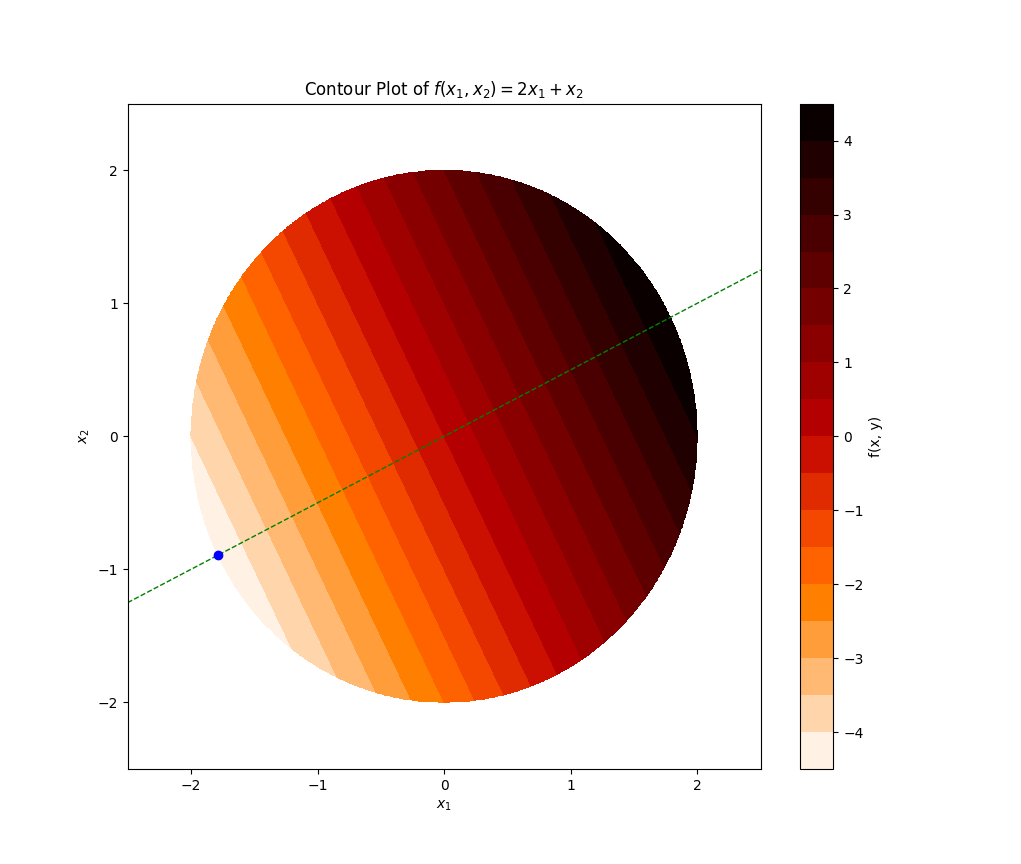
\includegraphics[scale=0.6]{ex1_solution.png}
\caption{Solución gráfica del problema.}
\label{ex1_solution}
\end{figure}

\subsection*{(b)}

El problema dual de $(P)$ se puede escribir como
\begin{equation*}
    \max_{u \geq 0} \inf_{(x_1, x_2) \in \R^2} 2 x_1 + x_2 + u ( x_1^2 + x_2^2 - 4 ).
\end{equation*}


\subsection*{(c)}

En el caso en que $x_1^2 + x_2^2 > 4$ entonces cuando $u \rightarrow \infty$ el valor del problema tiende a $\infty$,
si $x_1^2 + x_2^2 \leq 4$ entonces el máximo se alcanza cuando $u = 0$.
Por tanto el problema dual es equivalente al primal
\begin{equation*}
\begin{aligned}
    (D) \quad \inf \quad & 2 x_1 + x_2 \\
    \text{sujecto a} \quad & x_1^2 + x_2^2 \leq 4, \\
\end{aligned}
\end{equation*}
y sus valores óptimos coinciden.

Para encontrar el valor optimo,
planteamos el sistema de condiciones KKT
\begin{equation*}
\begin{aligned}
    2 + 2 u_1 x_1 & = 0, \\
    2 + 2 u_1 x_2 & = 0, \\
    x_1^2 + x_2^2 - 4 & = 0, \\
    u_1 \geq 0,
\end{aligned}
\end{equation*}
de la primera ecuacion tenemos que $x_1 = -\frac{1}{u_1}$ de la segunda $x_2 = -\frac{1}{2 u_1}$,
substituyendo en la tercera igualdad
\begin{equation*}
    \frac{1}{u_1^2} + \frac{1}{4 u_1^2} - 4 = 0
    \Rightarrow u_1 = \frac{\sqrt{5}}{4},
\end{equation*}
por tanto $\left( -\frac{4}{\sqrt{5}}, -\frac{2}{\sqrt{5}} \right)$ es un mínimo del problema,
como la función $f(x_1, x_2) = 2 x_1 + x_2$ es afín y la función $g_1(x_1, x_2) = x_1^2 + x_2^2 - 4$ es convexa,
por el Teorema 5.17 del libro de texto $\left( -\frac{4}{\sqrt{5}}, -\frac{2}{\sqrt{5}} \right)$ es solución del problema con valor $-\frac{10}{\sqrt{5}}$.

	\section*{2}

Determine la solución (máximo) del problema dual asociado al siguiente problema primal
\begin{equation*}
\begin{aligned}
    (P) \quad \min \quad & x_1 + 2 (x_2 - 1)^2 \\
    \text{sujecto a} \quad & - x_1 - x_2 + 1 \leq 0, \\
        & x_1, x_2 \in \R.
\end{aligned}
\end{equation*}

\noindent\rule{10cm}{0.4pt}

El problema dual asociado a $(P)$ se puede escribir como
\begin{equation*}
    \max_{u \geq 0} \inf_{(x_1, x_2) \in \R^2} x_1 + 2 (x_2 - 1)^2 - u (x_1 + x_2 - 1),
\end{equation*}
que es equivalente a
\begin{equation*}
    \max_{u \geq 0} \inf_{(x_1, x_2) \in \R^2}
        2 x_2^2
        - 4 x_2 
        + 2
        + u (1 - x_2)
        + (1 - u) (x_1),
\end{equation*}
vemos que si  $u < 1$ y $x_1 \rightarrow - \infty$ la function anterior tiende a $-\infty$,
por tanto $u \geq 1$,
pero si $u > 1$ entonces el ínfimo se alcanzaría cuando $x_1 \rightarrow \infty$ valiendo $-\infty$,
de modo que $u = 1$.
Y tenemos el problema
\begin{equation*}
    \min_{(x_1, x_2) \in \R^2}
        2 x_2^2
        - 5 x_2 
        + 3,
\end{equation*}
que tiene como mínimo $-\frac{1}{8}$,
y por tanto la solución del problema dual es $-\frac{1}{8}$.

\end{document}